% TFG - José Ángel Martín Baos. Escuela Superior de Informática. 2017
%%%% CHAPTER: Methodology %%%
\chapter{Methodology}
\label{chap:methodology}

% TODO: Revise all (English and content)

\drop{I}{n} order to carry out this project, a working methodology should be choosen and followed throughout the development of this \ac{TFG}. In particular, Scrum has been used as project management methodology and Kanban to manage the progress of the project. The details of the different means and resources that has been used are also described.


\section{Agile methodologies}

In the last few years, the number of companies of different size and from different areas which are using agile development methodologies has increased. These methodologies are not only used by the software development companies, but they are used by any kind of company. In the software engineering field, agile methodologies gain a lot of importance due to the complexity sometimes required to specify the different requirements of a product in a unique phase. The agile methodologies makes a great difference with respect to Waterfall model, where carry out a change once the product is almost finished is very costly.

In a agile project it is sought to divide the task of the software project in increments with a minimum planning and a short duration (normally between 1 and 4 weeks). Each iteration produces an operational prototype that is revised together with the client. Therefore, we can say that the life cycle of the agile methodologies is iterative and incremental.

Some examples of agile methodologies are:
\begin{multicols}{2}
	\begin{itemize}
		\item Scrum
		\item Adaptive Software Development
		\item Extreme Programming (XP)
		\item Open Unified Process (OpenUP)
		\item Feature-Driven Development
		\item Lean
	\end{itemize}
\end{multicols}

The \emph{11th anual state or agile survey} \cite{AnualStateAgile} (elaborated in April 2017) has elaborated a listing with the most used agile methodologies which can be seen in Figure \ref{fig:5-AgileMethodologyUsed}. The most used agile methodology is Scrum which is used by the 58\% of the organizations that use agile methodologies. 

Due to the fact that is the most used agile methodology and that it fits perfectly with the problem dealt in this \ac{TFG}, Scrum has been choosen. Specifically, Scrum methodology \cite{ScrumGuide} has been adapted to an unipersonal development. To manage the progress of the project graphically use the Kanban technique with the tool Trello.\footnote{Trello website: \url{www.trello.com} \label{footnote-1}}

\begin{figure}[!h]
	\begin{center}
		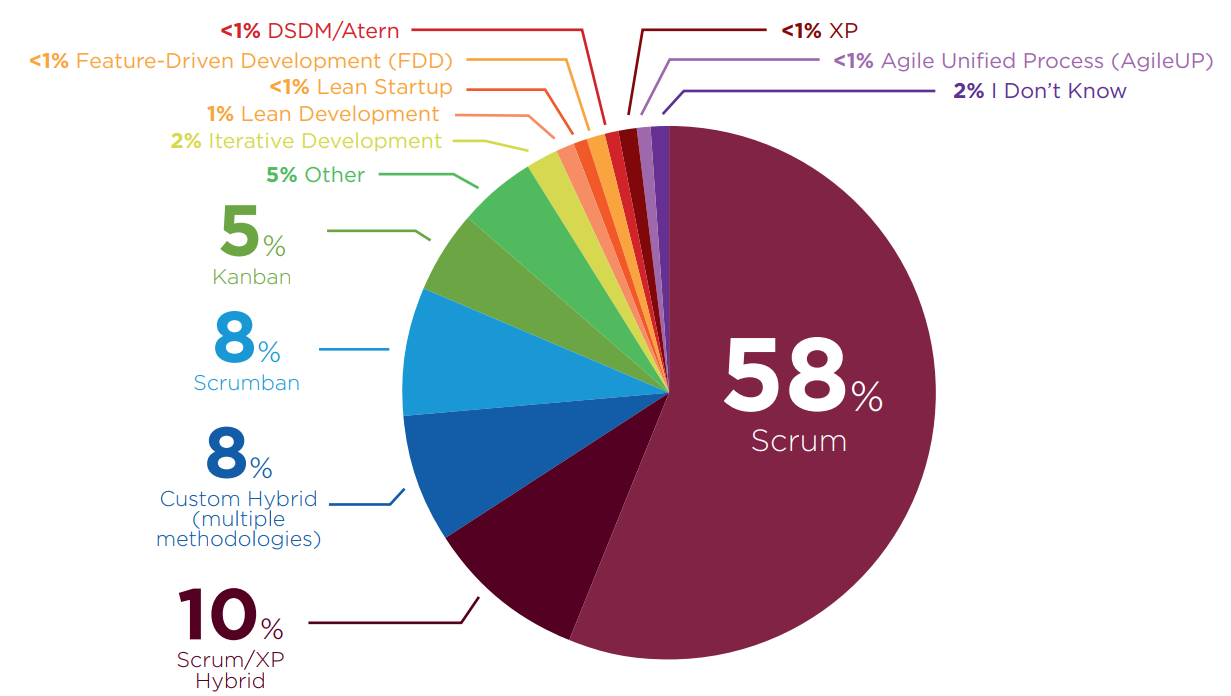
\includegraphics[width=1\textwidth]{5-AgileMethodologyUsed.png}
		\caption{More used agile methodologies.}
		\label{fig:5-AgileMethodologyUsed}
	\end{center}
\end{figure}


\subsection{Scrum}

Scrum \cite{ScrumGuide} is an agile project management methodology, but not necessarily related with software projects. Scrum has two main characteristics: The development of the software is carried out in incremental iterations and coordination meetings are held throughout the project.
Figure \ref{fig:5-ScrumSprints} represents the Scrum life cycle.\footnote{Image taken and modified from \url{https://www.visualstudio.com/es/learn/what-is-scrum}} In Scrum, the product is developed in series with a duration of 1 to 4 weeks called \emph{sprints}. The requirements are captured as elements of a list called \emph{product backlog}.

\begin{figure}[!h]
	\begin{center}
		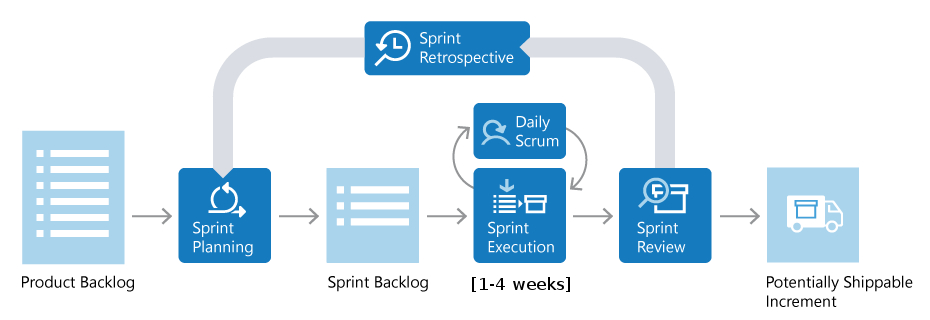
\includegraphics[width=1\textwidth]{5-ScrumSprints.png}	
		\caption{Scrum life cycle.}
		\label{fig:5-ScrumSprints}
	\end{center}
\end{figure}


\subsubsection{Scrum Team} \label{5-ScrumTeam}
Scrum Teams are self-organizing, cross-functional, non-distributed and with an optimal size. The team model in Scrum is designed to optimize flexibility, creativity, and productivity. The different roles in Scrum are:

\begin{itemize}
	\item Product Owner. Is responsible for maximizing the value of the product and the work of the	Development Team. This person is also responsible of establishing the user stories, assigning them a priority and classifying them in the Product Backlog. The product Owner must have a very clear perspective of the product which will be developed and must transmit it to the development team.
	
	\item Scrum Master. Is responsible for ensuring Scrum is understood and enacted. Scrum Masters do this by ensuring that the Scrum Team adheres to Scrum theory, practices, and rules. 
	
	\item Development Team. Consists of professionals who do the work of delivering a potentially releasable Increment of “Done” product at the end of each Sprint. It is recommended that they work full time, in the same place and they should not change during a sprint.
\end{itemize}


\subsubsection{The Sprint}

In agile methodologies, the requirements that must fit the software which will be developed are collected into user stories. The user stories are a brief description of the software functionality as the user perceives them. \cite{Coh04} A Sprint is a time bloc with a duration of one to four weeks in which a product increment is obtained. A new Sprint starts immediately after the conclusion of the previous Sprint. During the Sprint no changes are made that would endanger the Sprint Goal (objective set for the Sprint that can be met through the implementation of Product Backlog). Each Sprints can be considered as a project itself, with a duration, as mentioned previously, between one and 4 weeks.


\subsubsection{Scrum Events}
Some events are planned when using Scrum with a fixed duration and concrete objective in order to minimize the need for meetings not defined. These events are the following ones:

\begin{itemize}
	\item Sprint planning meeting. Consists on a meeting realized at the start of each Sprint where the elements from the Product Backlog that will be developed are selected. Therefore, the Sprint Backlog is created. It should not last more than one day.
	
	\item Daily Scrum. Consist on daily meetings with a duration of less than fifteen minutes where the development team can synchronize their activities and create a plan for the next 24 hours. This is done by inspecting the work since the last Daily Scrum and forecasting the work that could be done before the next one.
	
	\item Sprint Review. Consist on a informal meeting held at the end of the Sprint to inspect the Increment and adapt the Product Backlog if needed. During the Sprint Review, the Scrum Team and stakeholders collaborate about what was done in the Sprint.
	
	\item Sprint Retrospective. It is an opportunity for the Scrum Team to inspect itself and create a plan for improvements to be enacted during the next Sprint. It has a maximum duration of three hours and takes places between the Sprint Review meeting and the next Sprint planning meeting.
\end{itemize}


\subsubsection{Scrum Artifacts}
When using Scrum, some outputs are obtained known as Artifacts. They represent work or value to provide transparency and opportunities for inspection and adaptation. In Figure \ref{fig:5-ScrumSprints} it can be shown the different artifacts and when are they obtained.

\begin{itemize}
	\item Product Backlog. Consist on an ordered list of requirements or user stories that will be included in the software product in the increments. This list is created by the Product Owner. This list is never complete, therefore, it can change during the project to identify what the product needs. 
	
	\item Sprint Backlog. It is a subset of the elements contained in the Product Backlog. Consist on an ordered list of user stories that will be developed during this Sprint.
	
	\item Product increment. The Increment is the sum of all the Product Backlog items that has been completed during a Sprint and the value of the increments of all the previous Sprints.
\end{itemize}


\section{Kanban}

Kanban \cite{Gar11,KS10} is a Japanese technique for managing the progress of the project. It was invented by Toyota and was used to control de progresses of their work in the production line. Therefore, Kanban is not a specific software development technique, nevertheless, in the last few years it has been used in the management of software projects.

Kanban allows the development team to visualize the workflow of the different task. Normally, consists on using a slate board with three colums: \emph{To Do}, \emph{Doing} and \emph{Done}, which represents the different phases that a task passes until it has been completed. Each task in which a sprint is divided is considered as a card which is put into the slate board. An example of this concept can be seen in Figure \ref{fig:5-KanbanBoard}.\footnote{Image from \url{www.qe2ingenieria.com}}

To manage the Kanban Board Trello has ben used, as it was previously commented. This tool allow creating several boards. In each board many columns can be created with various task that can be moved from one column to another using a very friendly interface.

\begin{figure}[!h]
	\begin{center}
		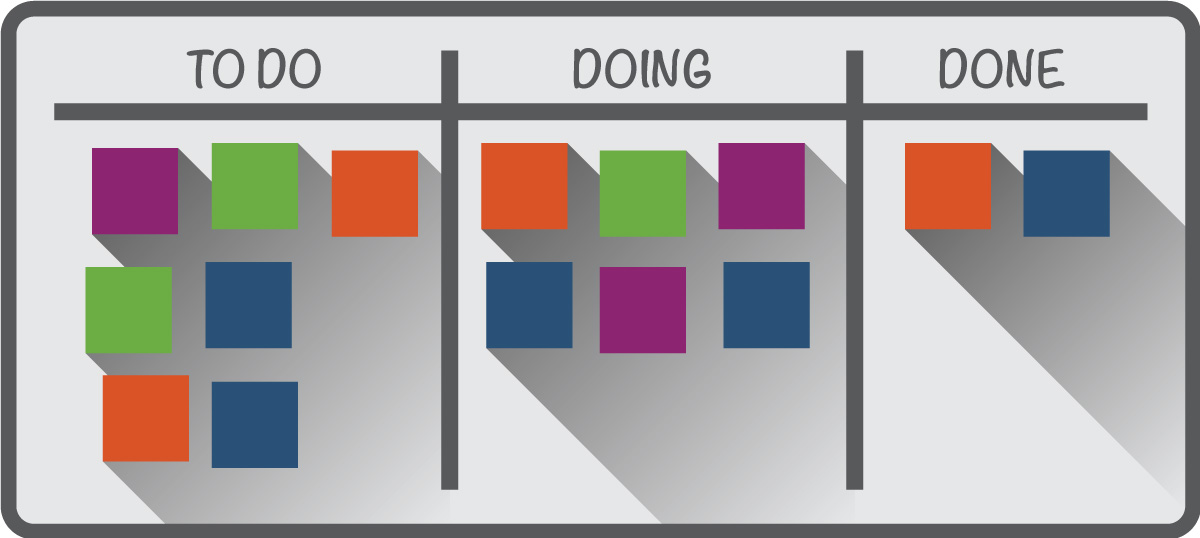
\includegraphics[width=0.8\textwidth]{5-KanbanBoard.jpg}
		\caption{Kanban Board.}
		\label{fig:5-KanbanBoard}
	\end{center}
\end{figure}





\REDNOTE{UML ?}


\section{Resources} %TODO: Completar
In this section we are going to describe the different technologies that will be employed during the development of this \ac{TFG}.

\subsection{Hardware resources}
In this part the different hardware resources employed in the \ac{TFG} are detailed. This includes the computer used to develop the \ac{TFG}, the Raspberry Pi and the different peripherals attached to it.

\begin{itemize}
	\item \textbf{Development computer.} The personal computer of the student has been employed for this purpose. The spec table can be shown in Table \ref{tab:development-computer-spec-table}.
	
	\begin{table}[hp]
		\centering
		{\small
			\begin{tabular}{ |l|l|}
	\hline
	\rowcolor{tabheadbg}
	\multicolumn{2}{|c|}{\textscale{.8}{\textbf{Development computer (\emph{draco}) specs}}} \\
	\hline
	Model						& Asus Zeenbook UX430UA \\
	\hline
	Processor					& Intel® Core™ i7-7500U CPU at 2.70GHz $\times$ 4 \\
	\hline
	RAM memory 					& 8 GB \\
	\hline 
	Hard drive					& 512 GB HDD \\
	\hline
	First Operating System		& Ubuntu 16.04.3 LTS \\
	\hline
	Second Operating System		& Windows 10 \\
	\hline

\end{tabular}
		}
		\caption{Development computer spec table}
		\label{tab:development-computer-spec-table}
	\end{table}
	
	\item \textbf{Raspberry Pi 3.} The Raspberry Pi is a low cost, credit-card sized computer. The Raspberry Pi 3 is the third-generation Raspberry Pi. Table \ref{tab:raspberry-pi3-spec-table} shows its spec table. With this computer a memory card is also needed. The one used is \emph{Samsung SDHC EVO 8gb Class 10+}.
	
	\begin{table}[hp]
		\centering
		{\small
			%\begin{tabular}{ |l|l|l|}
%	\hline
%	\rowcolor{tabheadbg}
%	\multicolumn{3}{|c|}{\textscale{.8}{\textbf{Raspberry Pi 3 Model B specs}}} \\
%	\hline
%	Price						& $\sim$35\euro{} \\
%	\hline
%	SoC							& Broadcom BCM2837 \\
%	\hline
%	Processor					& Quad Core ARM Cortex A53 (ARMv8) at 1.2GHz 64bit \\
%	\hline
%	RAM memory 					& 1 GB \\
%	\hline 
%	GPIO pins					& 40 \\
%	\hline
%	\multirow{7}{*}{External ports}
%		& HDMI \\ 
%		& CSI camera port \\ 
%		& DSI display port \\ 
%		& Micro SD port \\
%		& 4 $\times$ USB 2 ports \\
%		& Ethernet port \\
%		& Audio jack 3,5 mm \\
%	\hline
%	\multirow{2}{*}{Wireless connections}
%	& BCM43438 wireless LAN  \\ 
%	& Bluetooth Low Energy (BLE) \\
%	\hline
%
%\end{tabular}

\begin{tabular}{ |l|l|l|}
	\hline
	\rowcolor{tabheadbg}
	\multicolumn{3}{|c|}{\textscale{.8}{\textbf{Raspberry Pi 3 Model B specs}}} \\
			\hline
	Price                                 & $\sim$35\euro{}                                  & \multirow{14}{*}{
		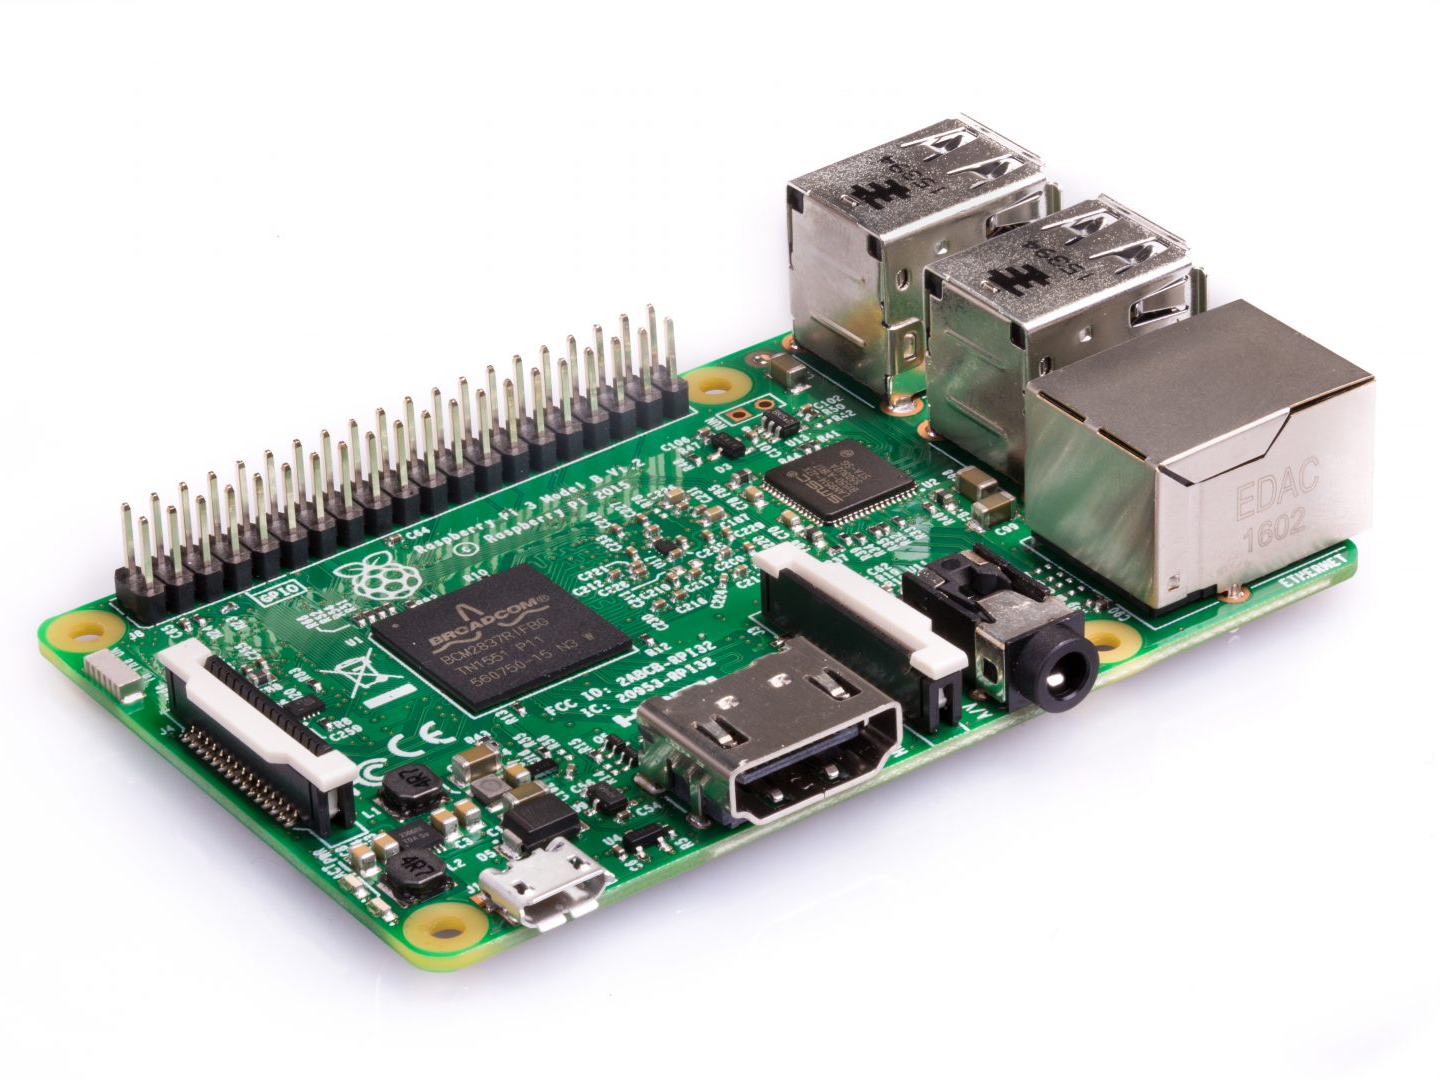
\includegraphics[width=0.36\textwidth]{5-RaspberryPi3.jpg}
	} \\ \cline{1-2}
	SoC                                   & Broadcom BCM2837                                 &                         \\ \cline{1-2}
	Processor                             & Quad Core ARM Cortex A53 				 &                         \\ 
			                              & (ARMv8) at 1.2GHz 64bit 								 &                         \\ \cline{1-2}
	RAM memory                            & 1 GB                                             &                         \\ \cline{1-2}
	GPIO pins                             & 40                                               &                         \\ \cline{1-2}
	\multirow{7}{*}{External ports}       & HDMI                                             &                         \\
	& CSI camera port                                  &                         \\
	& DSI display port                                 &                         \\
	& Micro SD port                                    &                         \\
	& 4 × USB 2 ports                                  &                         \\
	& Ethernet port                                    &                         \\
	& Audio jack 3,5 mm                                &                         \\ \cline{1-2}
	\multirow{2}{*}{Wireless connections} & BCM43438 wireless LAN                            &                         \\ \cline{2-2}
	& Bluetooth Low Energy (BLE)                       &                         \\ \hline
	
	
\end{tabular}

		}
		\caption{Raspberry pi 3 spec table}
		\label{tab:raspberry-pi3-spec-table}
	\end{table}
	
	\item \textbf{Raspberry Pi Camera Module V2. \cite{PiCameraDoc}} Is a hardware module that allow the Raspberry Pi to capture pictures and record videos using the CSI port. The camera used is the \emph{PI NOIR CAMERA V2}.\footnote{More information in https://www.raspberrypi.org/products/pi-noir-camera-v2/} The table \ref{tab:raspberry-pi3-camera-specs} shows its specs. \label{itm:Pi-camera-module-v2}
	
	\begin{table}[hp]
		\centering
		{\small
			%\begin{tabular}{ |l|l|}
%	\hline
%	\rowcolor{tabheadbg}
%	\multicolumn{2}{|c|}{\textscale{.8}{\textbf{Pi NoIR Camera V2 specs}}} \\
%	\hline
%	Price						& $\sim$25\euro{} \\
%	\hline
%	Weight						& 3g \\
%	\hline
%	Resolution					& 8 Megapixels \\
%	\hline 
%	Dimensions					& 25$\times$24$\times$9 mm \\
%	\hline	
%	Sensor						& Sony IMX219 \\
%	\hline
%	\multirow{3}{*}{Video modes}
%		& 1080$\times$120p at 30 fps \\ 
%		& 720$\times$480p at 60 fps\\ 
%		& 640$\times$480p at 60$/$90 fps \\ 
%	\hline
%	Additional information		& No Infrared filter (NoIR) \\
%	\hline
%\end{tabular}

% Please add the following required packages to your document preamble:
% \usepackage{multirow}


\begin{tabular}{|l|l|l|}
	\hline
	\rowcolor{tabheadbg}
	\multicolumn{3}{|l|}{\textscale{.8}{\textbf{Pi NoIR Camera V2 specs}}}                       \\ \hline
	Price                        & $\sim$25\euro{}                     & \multirow{9}{*}{
		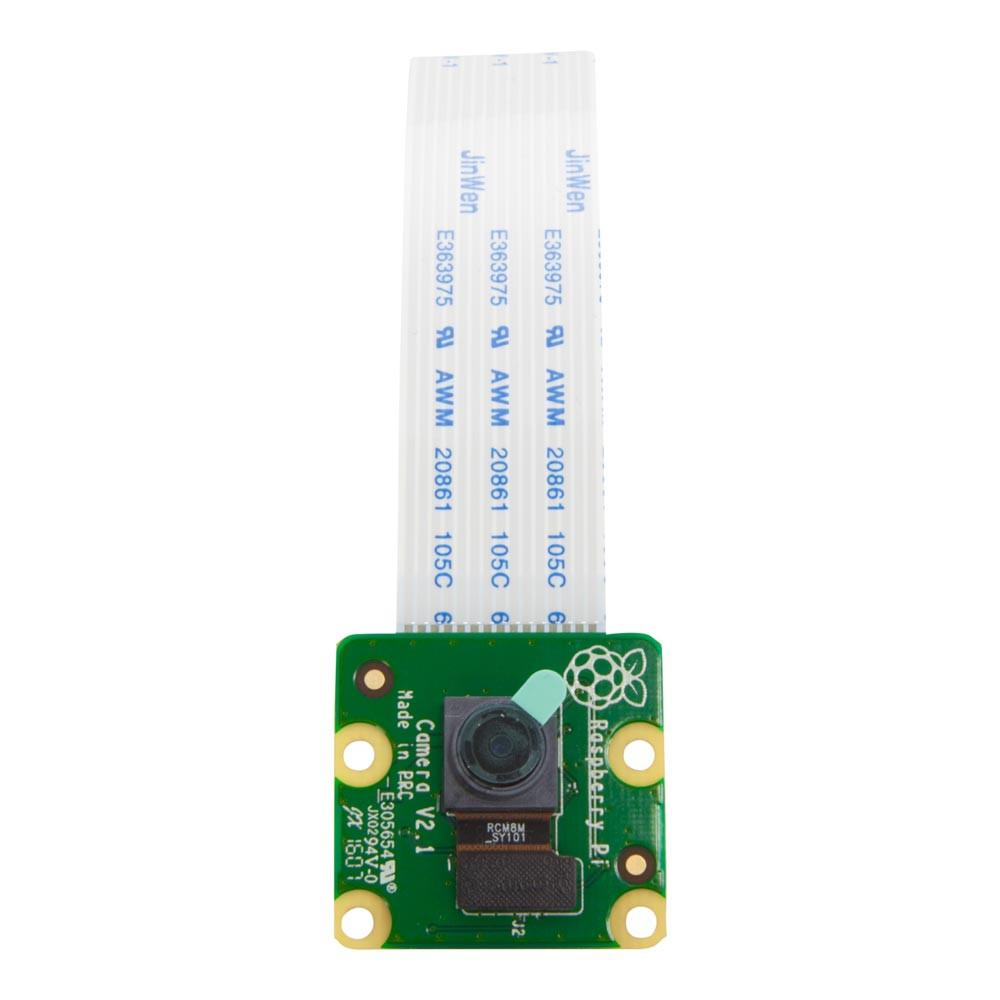
\includegraphics[width=0.28\textwidth]{5-PiCamera.jpg}
	} \\ \cline{1-2}
	Weight                       & 3g                        &                   \\ \cline{1-2}
	Resolution                   & 8 Megapixels              &                   \\ \cline{1-2}
	Dimensions                   & 25×24×9 mm                &                   \\ \cline{1-2}
	Sensor                       & Sony IMX219               &                   \\ \cline{1-2}
	\multirow{3}{*}{Video modes} & 1080p at 30 fps           &                   \\
	& 720p at 60 fps            &                   \\
	& 640x480p at 60/90 fps     &                   \\ \cline{1-2}
	Additional information       & No Infrared filter (NoIR) &                   \\ \hline
\end{tabular}
		}
		\caption{Pi NoIR Camera V2 spec table}
		\label{tab:raspberry-pi3-camera-specs}
	\end{table}
	
	\item \textbf{\REDNOTE{Power bank battery.}}
	
	
	
	\item \textbf{\REDNOTE{Internet connection.}}
	
	
	
	\item \textbf{\REDNOTE{Sensors.}}
	
	
	
\end{itemize} 



\subsection{Software resources}
In this part the different software resources employed are described. This include the \ac{OS}, programming languages, libraries, the different development tools and the software used for the documentation.

\REDNOTE{Image of the different software resources as in DanielEsteban \ac{TFG}.} %TODO

\textbf{Operating Systems:}
\begin{itemize}
	\item \textbf{Ubuntu 16.04.3 LTS.} Ubuntu is a popular \ac{OS} based on \ac{GNU}$/$Linux. Ubuntu is one of the most used Linux distributions and it is normally used for personal computers, but also for servers and \ac{IoT}. This \ac{OS} will be used for developing the software in the student computer.
	
	\item \textbf{Debian 9 “Stretch”.} Debian is also a \ac{OS} based on \ac{GNU}$/$Linux. Debian has a big community form by developers and users, which maintain the software. It will be used also for developing the software.
	
	\item \textbf{Raspbian.} Raspbian is a Debian-based \ac{OS} designed for running in the Raspberry Pi.
	
	
\end{itemize}

\textbf{Programming Languages:}
\begin{itemize}
	\item \textbf{Python 3 \cite{Dow12}.} Python is a high-level programming language. Python focuses on offering a simple syntax, as well as being an interpreted language, allowing it to be ideal for scripting and for developing applications in various areas and for most platforms. In addition, it is an \ac{OO} language and has efficient and high-level data structures. Python has been used because it has lot of support for Raspberry Pi. Moreover, the main libraries for the camera module of the Raspberry Pi are written in Python and can use the power of the NumPy scientific computation library.
	
\end{itemize}

\textbf{Libraries:}
\begin{itemize}
	\item \textbf{Python PiCamera \cite{PiCameraDoc}.} Python library for Python 2.7 or Python 3.2 (or above) which provides an interface for controlling the Raspberry Pi camera (PiCamera described in \ref{itm:Pi-camera-module-v2}).
	
	\item \textbf{Python NumPy \cite{NumPy}.} NumPy is a open-source scientific computing package for Python. It provides an easy and efficient way of working with multidimensional structures, such as the matrices of motion vectors used by H.264/AVC video format that is employed by the PiCamera library.
	
	\item \textbf{Python Matplotlib \cite{Hun07}.} Matplotlib is a Python 2D plotting library which produces quality figures in a variety of formats. For simple plotting the \emph{pyplot} module provides a MATLAB-like interface.
	
\end{itemize}

\textbf{Development tools:}
\begin{itemize}
	\item \textbf{Atom.} Atom is a free open-source text and source coder editor for macOS, Linux and Windows developed by GitHub. It allows to install a lot of plug-ins writen in Node.js and has and embedded Git Control tool.\footnote{Available at \url{https://atom.io/}}
	
	\item \textbf{Vi.} Vi is a console text editor originaly created for the Unix \ac{OS}. 
	
	\item \textbf{Git \cite{CS14}.} Git is a version control system for tracking changes in computer files and coordinating work on those files among multiple people. It is primarily used for source code management in software development, but it can be used to keep track of changes in any set of files.
	
	\item \textbf{GitHub.} GitHub is a web-based Git version control repository. It provides access control and several collaboration features such as bug tracking, feature requests, task management, and wikis for every project.\footnote{GitHub webpage: \url{https://github.com/}}
	
	%\item \textbf{Make}    https://www.gnu.org/doc/doc.html
	
	
\end{itemize}

\textbf{Software used for the documentation:}
\begin{itemize}
	\item \textbf{Trello.} Trello is a web tool which provides support for the Kanban technique allowing to manage the progress of the project. Trello provides the functionality to create boards composed by several lists with cards in them. For this project, a board has been created with 3 lists: \emph{To Do}, \emph{Doing} and \emph{Done}.$^{\ref{footnote-1}}$
	
	\REDNOTE{Insert a screen capture of the Board} %TODO
	
	\item \textbf{\LaTeX{} \cite{Kot11}.} \LaTeX{} is a software for typesetting documents. It is not a word processor, but is used as a document markup language. \LaTeX{} is free, open source and provide great typographic quality on the documents, which makes it ideal for composing scientific documents. It is based on the \TeX{} typesetting engine created by Donald Knuth.
	
	\item \textbf{TeXstudio.} TeXstudio is a cross-platform and open source \LaTeX{} editor. TeXstudio has numerous features like syntax-highlighting, integrated viewer, reference checking, code folding and various assistants. Originally, TeXstudio was started as a fork of Texmaker that tried to extend it with additional features. 
	
	\item \textbf{esi-tfg \LaTeX{} class.} It is a \LaTeX{} class with allows to write the \ac{TFG} in a simple way, as its format conforms to the specification established for the \ac{TFG} by the \emph{Escuela Superior de Informática} from Ciudad Real. This class can be downloaded from the Arco Research Group Bitbucket page.\footnote{Available at \url{https://bitbucket.org/arco_group/esi-tfg}}
	
	\item \textbf{GIMP.} GIMP (\ac{GNU} Image Manipulation Program) is a free and open-source raster graphics editor used for image editing.
	
	%\item \textbf{Inkscape.}
	
\end{itemize}

\textbf{Additional software:}
\begin{itemize}
	\item \textbf{MP4Box \cite{MP4Box}.} MP4Box is the multimedia package available in GPAC. It can be used for performing manipulations on multimedia files such as AVI, MPG, TS and ISO media files (for example MP4 or 3GP). In this work, it has been used to generate MP4 files from H.264 video format.
	
	%TODO: Add more additional software	
	
\end{itemize}
